\chapter{Results}
\vspace{-0.75cm}

The estimator developed in this project estimates the activity of a \ac{TF} over time from the expression of the genes it is believed to regulate. It does so by applying \ac{PCA} to the data to acquire a variable represents the \ac{TF}'s activity. 

The estimator was tested using mRNA count data mapped to 32394 genes in \textit{M. musculus} brain and liver sampled at 15.5 and 18.5 days into embryonic development, as well as 0.5, 4, 22 and 29 days into postnatal development. The data from liver and brain were analysed separately. All genes with no expression at any sampling point were removed, which resulted in a reduction from 32394 genes to 14458 for the liver data and to 16338 for the brain data. Given the assumption that count data is log-normally distributed, and that \ac{PCA} works under the assumption that the data it is applied to is normally distributed, the data was log2-transformed. The resulting distribution can be seen in Figure \ref{fig:logdatadist} in the appendix.

For the 17 \acp{TF} whose gene expression had the highest variance among those with an above average mRNA expression in either mouse liver or brain, list of genes they likely regulate were fetched from ChIP-atlas. These were used to extract subsets of mRNA expression data, whose first \ac{PC} served as the estimation of the \acp{TF}' activities. As a form of validation of the estimations on the basis of there being a correlation between gene expression and protein activity, the activity estimations were plotted and compared to the mRNA expression of the gene coding for the \ac{TF} itself. The gene likely controls protein activity to a degree and was thus used to indicate if the estimator produced accurate results. It should however be recognized that the correlation between transcript level and protein activity was expected to be perfect far from perfect due to the various forms of post-transnational regulatory mechanisms. 

The estimations for the 17 selected \acp{TF} showed promising results in both brain and liver. High similarities could be seen between the activity estimations and mRNA expressions, as exemplified by the estimations for Sox11 in Figure \ref{fig:est_allPCs_Sox11}. The estimations for all 17 \acp{TF}' activities in brain can be seen in Figure \ref{fig:BrainEsts1} and \ref{fig:BrainEsts2} in the appendix, and the estimations for their activities in liver can be seen in Figure \ref{fig:LiverEsts1} and \ref{fig:LiverEsts2} in the appendix. Note that the \ac{PCA} does not differentiate between overall positive and negative change, so the inverted activity estimation along the Y-axis also had to be considered when compared to the mRNA expressions.

\begin{figure}
    \centering
    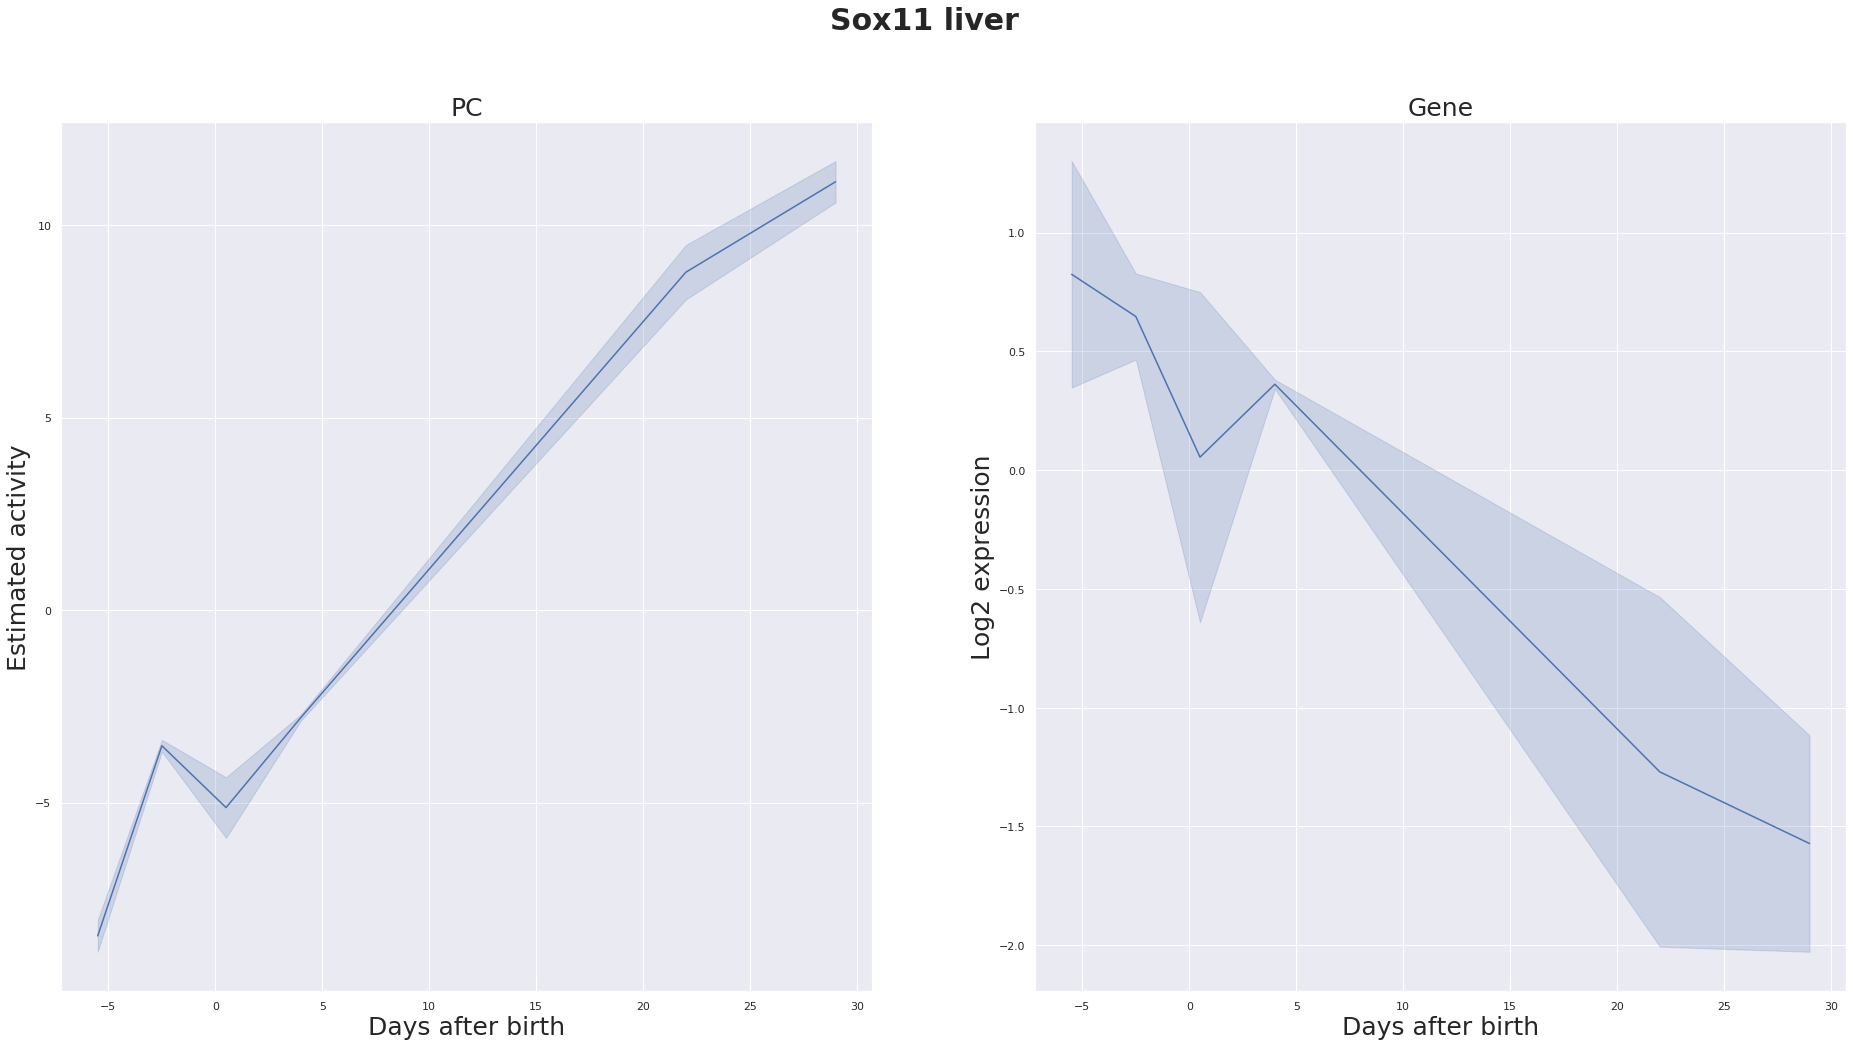
\includegraphics[width=11cm, height=5.5cm]{Figures&amp;Cover/Activity_Sox11_liver_NonePCremoved_filtering_False.png}
    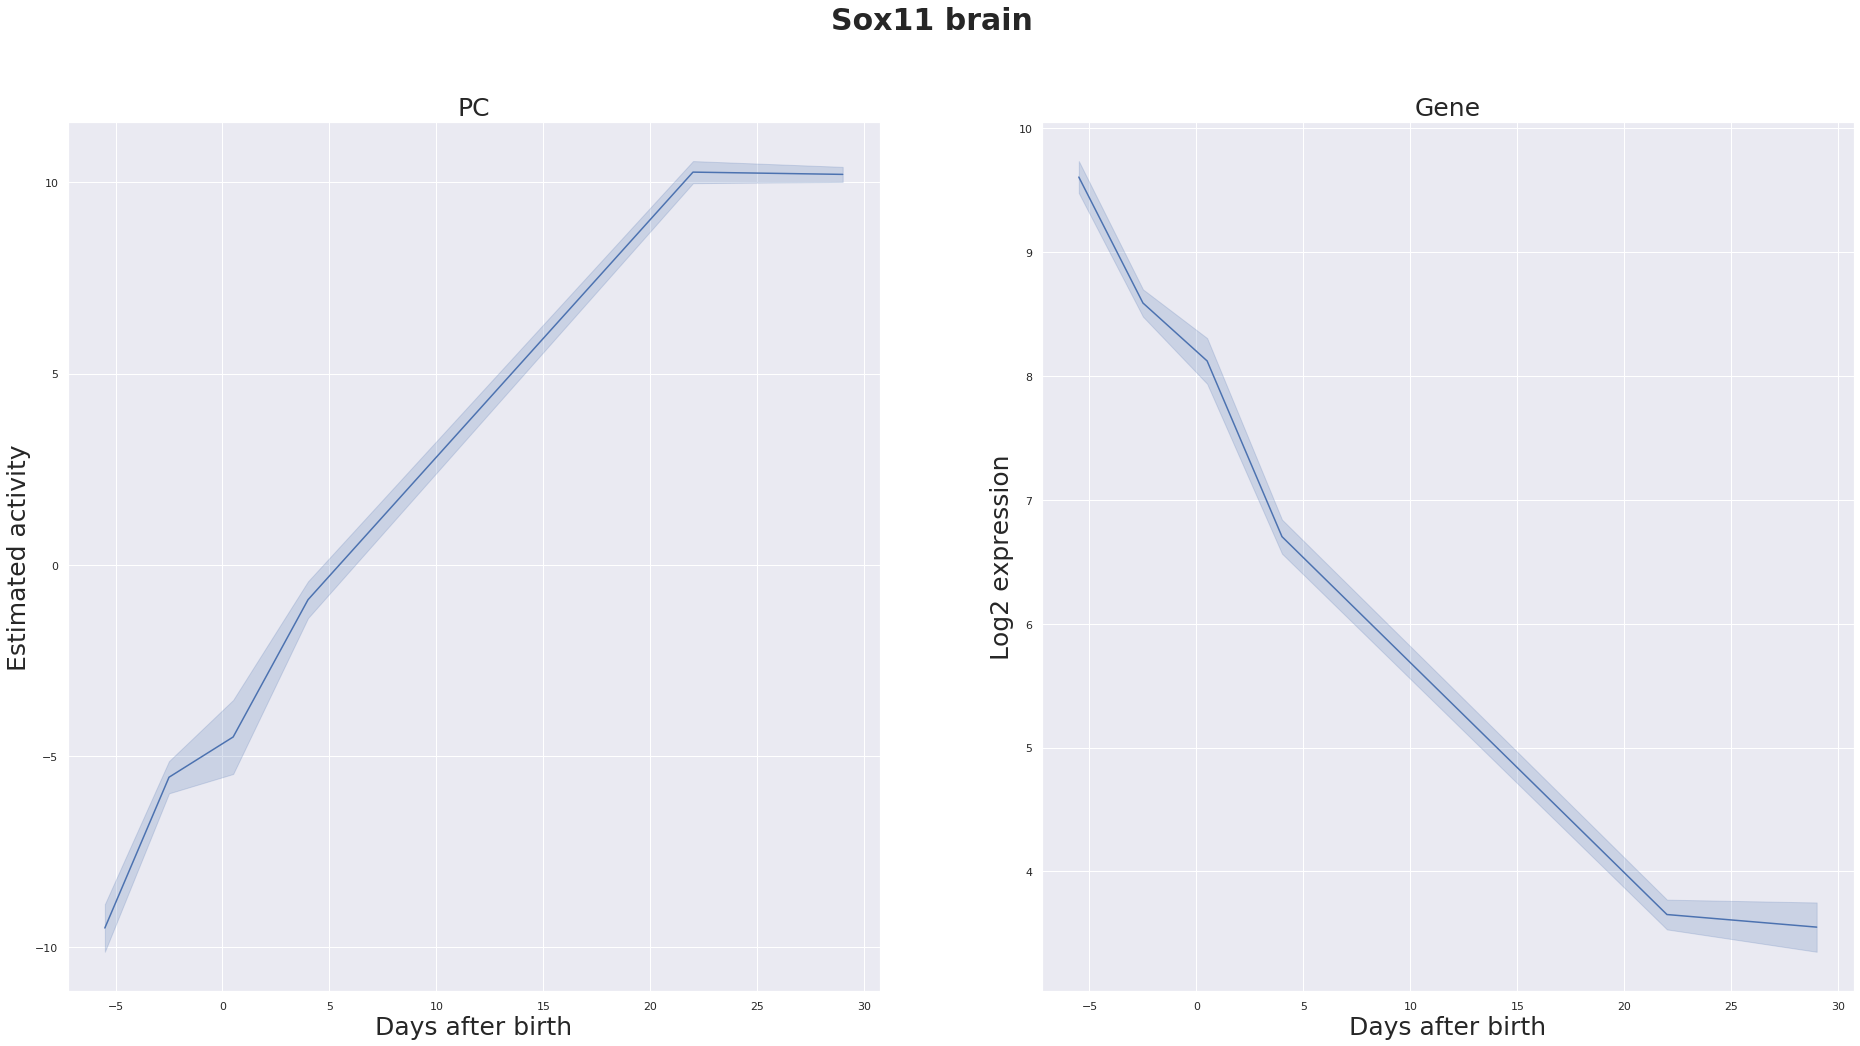
\includegraphics[width=11cm, height=5.5cm]{Figures&amp;Cover/Activity_Sox11_brain_NonePCremoved_filtering_False.png}
    \caption{\textbf{Sox11's estimated activity as a functions of mices' age.} Sox11's activity was estimated by the first \ac{PC} of the mRNA expression data of the genes it is likely to regulate (upper and lower left) as well as directly through the transcription of the genes coding for it, as log2-transformed gene count (upper and lower right). The activity estimations and mRNA expressions are from the data from mouse liver (upper left and right) and brain (lower left and right).}
    \label{fig:est_allPCs_Sox11}
\end{figure}

All of the 17 initially tested \acp{TF} shared similar trends in their activity estimations, with only slight variations. The same was true for the mRNA expressions of most \acp{TF}, but with a few exceptions as shown by the mRNA expression of Satb2 in Figure \ref{fig:est_allPCs_Satb2}. This was concerning as it indicated that the estimator was capturing a general trend in the data, possibly cause by a confounder, rather than patterns specific for the \acp{TF}. The percentage of total variance explained by the \ac{PC} used as activity estimation for each \ac{TF} was plotted, revealing that it ranged between 40-80\% and mostly clustered around 60\% for both brain and liver, as shown in Figure \ref{fig:VarExp_allPCs}. These high values further indicated that the genes measured had highly similar patterns of mRNA expression, supporting the theory of the presence of a confounder. To further investigate the existence of the trend, the first \ac{PC} for the full data set for each organ was plotted to be compared to the activity estimations and can be seen in Figure \ref{fig:firstPC}. These plots were for both organs highly similar, and their similarities to the activity estimations again indicated that there was a general trend in the data.

\begin{figure}
    \centering
    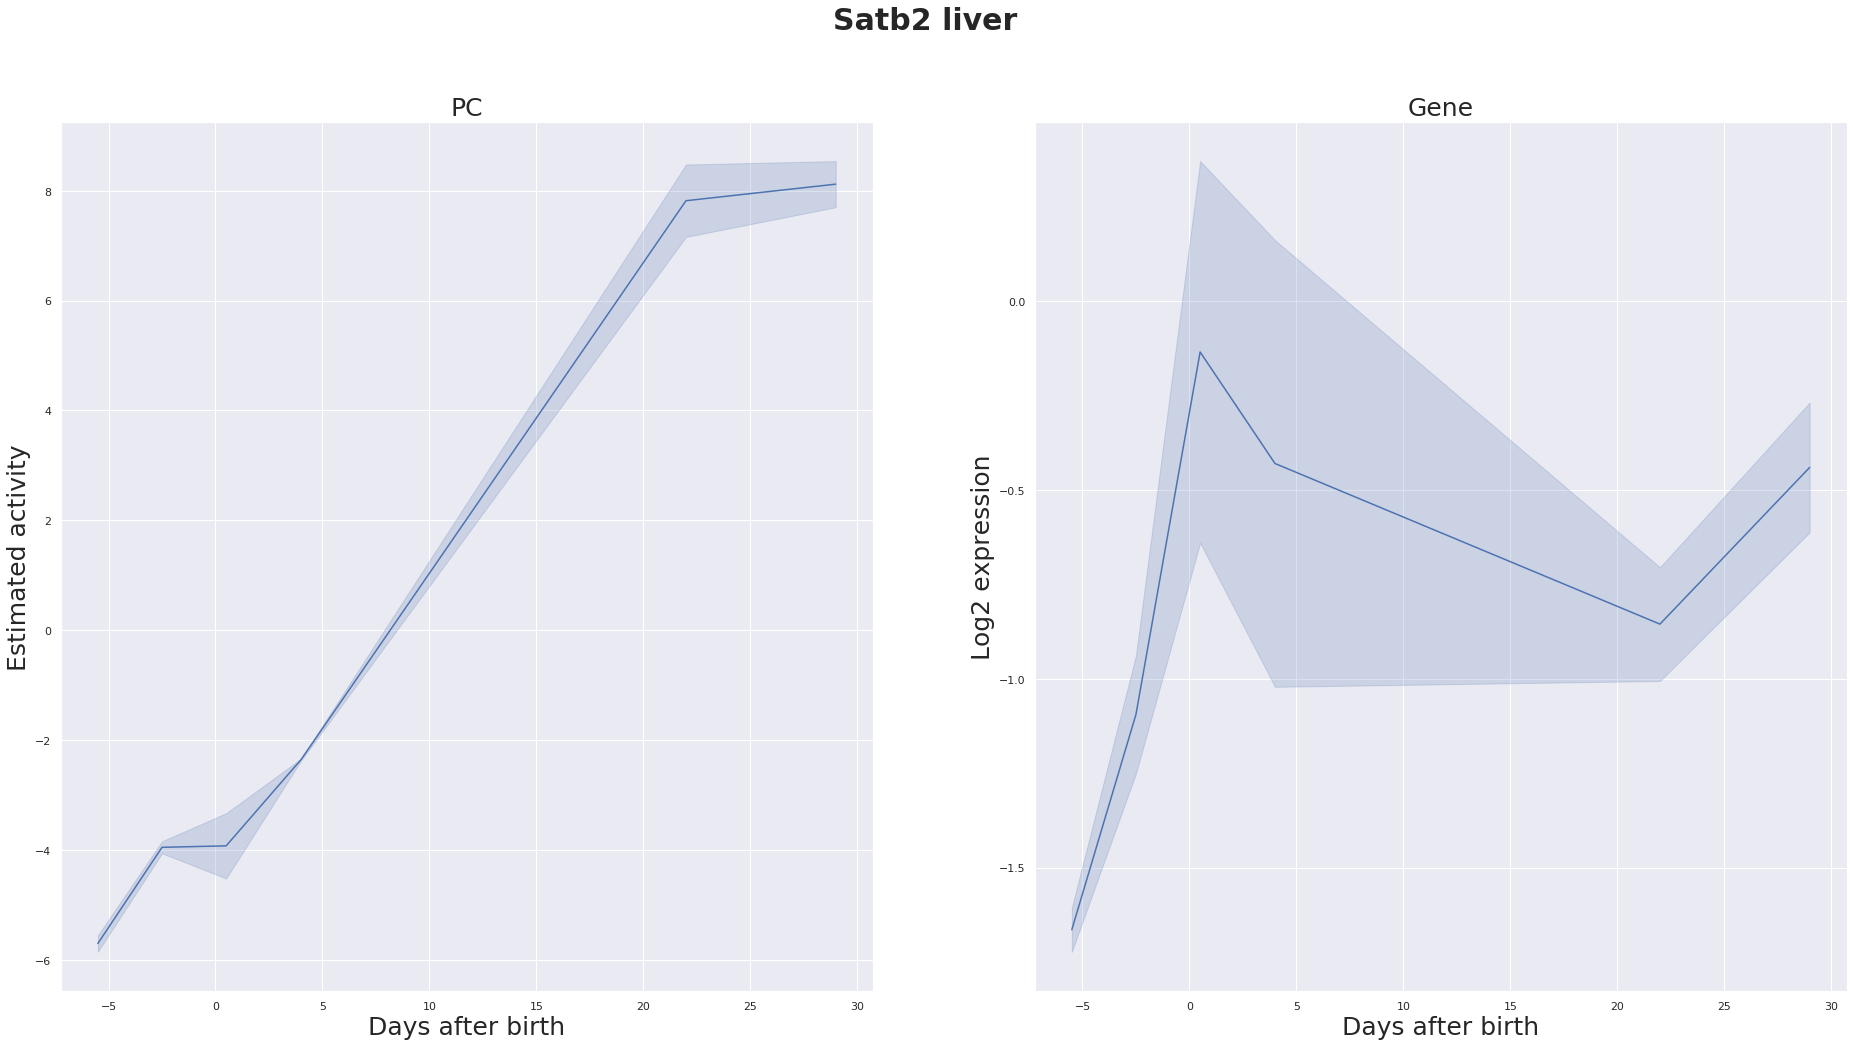
\includegraphics[width=11cm, height=5.5cm]{Figures&amp;Cover/Activity_Satb2_liver_NonePCremoved_filtering_False.png}
    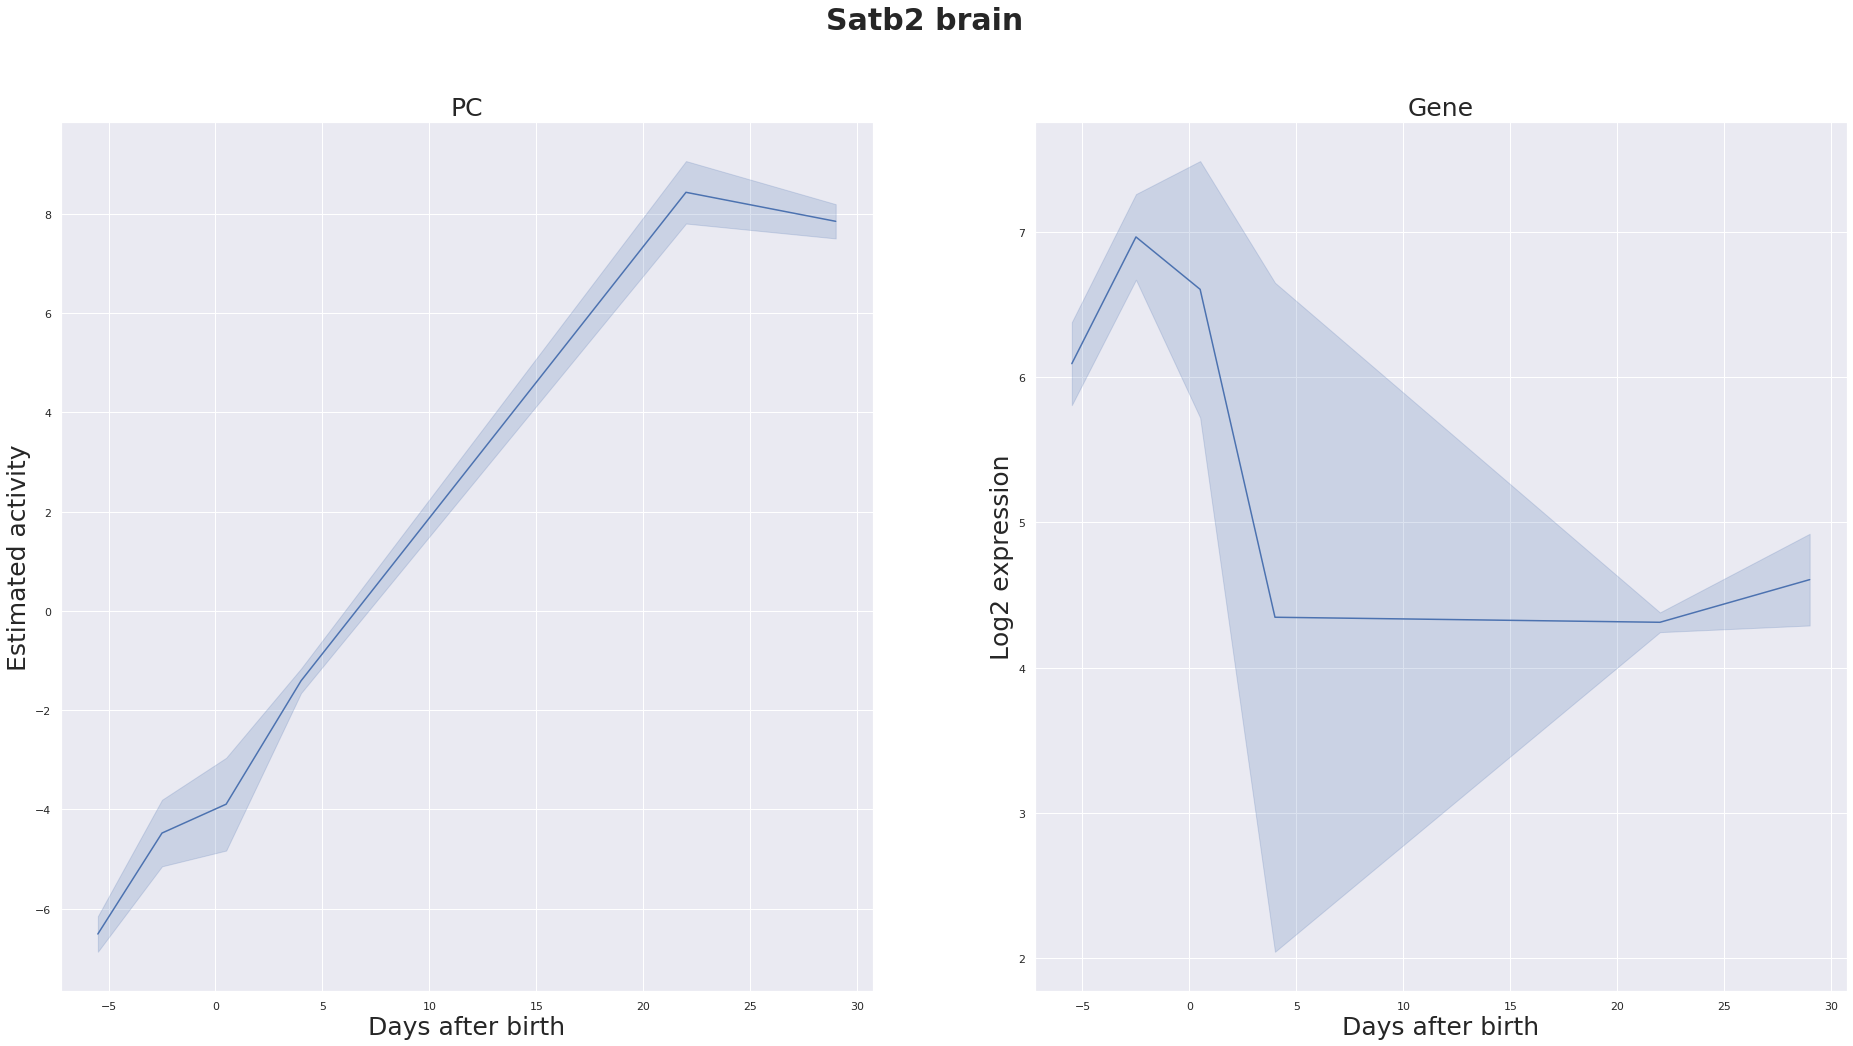
\includegraphics[width=11cm, height=5.5cm]{Figures&amp;Cover/Activity_Satb2_brain_NonePCremoved_filtering_False.png}
    \caption{\textbf{Satb2's estimated activity as a functions of mices' age.} Satb2's activity was estimated by the first \ac{PC} of the mRNA expression data of the genes it is likely to regulate (upper and lower left) as well as directly through the transcription of the genes coding for it, as log2-transformed gene count (upper and lower right). The activity estimations and mRNA expressions are from the data from mouse liver (upper left and right) and brain (lower left and right).}
    \label{fig:est_allPCs_Satb2}
\end{figure}

\begin{figure}
    \centering
    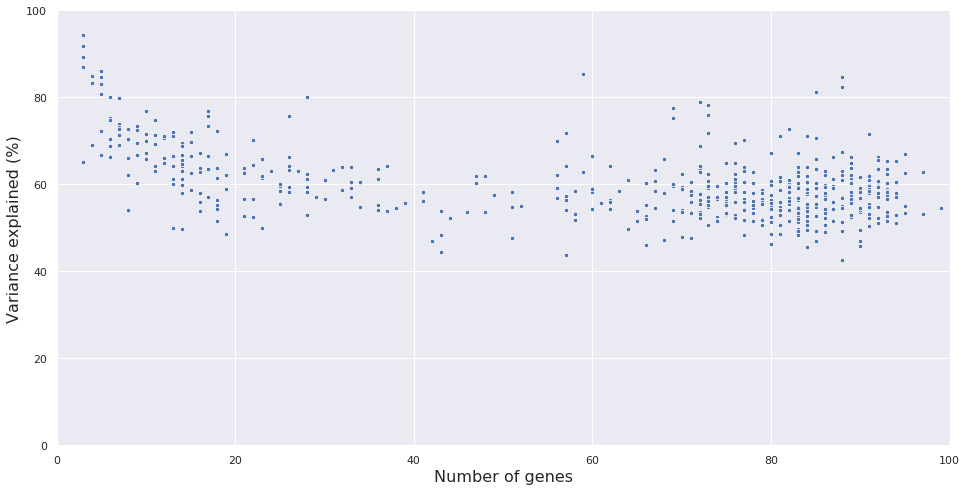
\includegraphics[width=10cm,height=5cm]{Figures&amp;Cover/VarExpl_PC1_10_300_100_liver_NonePCremoved_filtering_False.png}
    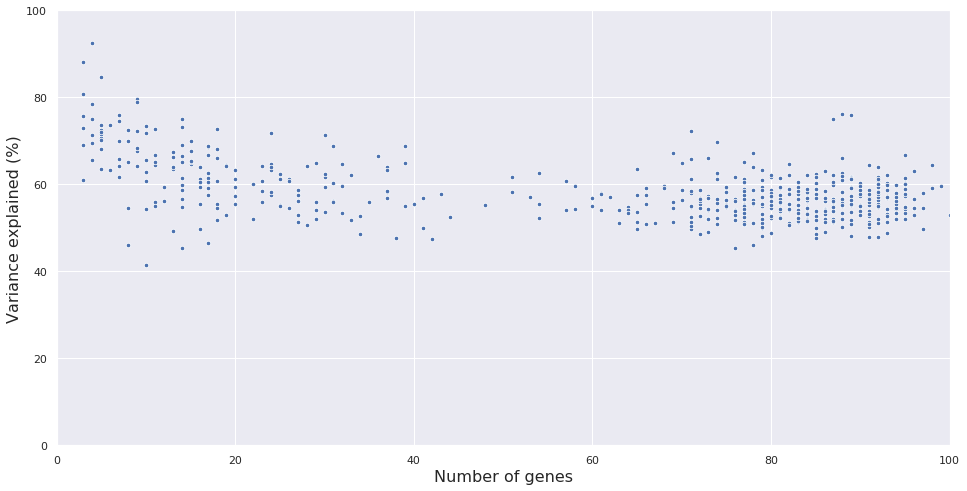
\includegraphics[width=10cm,height=5cm]{Figures&amp;Cover/VarExpl_PC1_10_300_100_brain_NonePCremoved_filtering_False.png}
    \caption{\textbf{The variance explained in the transcription data of the genes in each \ac{TF}'s gene set, as a function of the number of genes in the gene set.}  For the top plot the unmodified data from mouse liver was used and for the bottom plot the unmodified data from mouse brain. For both data sets, the first \ac{PC} is explained about 60\% of the variance, slightly more for smaller gene sets.}
    \label{fig:VarExp_allPCs}
\end{figure}

\begin{figure}
    \centering
    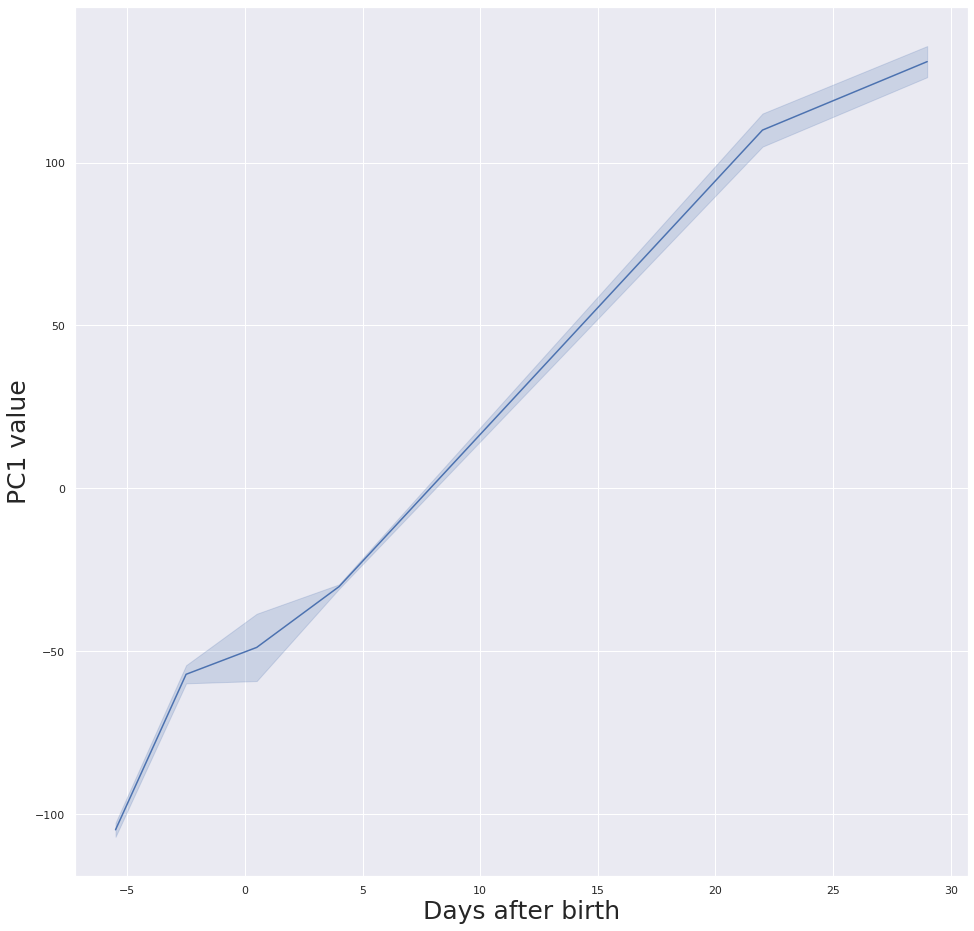
\includegraphics[width=5.5cm,height=5.5cm]{Figures&amp;Cover/Fulldata_liver_NonePCremoved_filtering_False.png}
    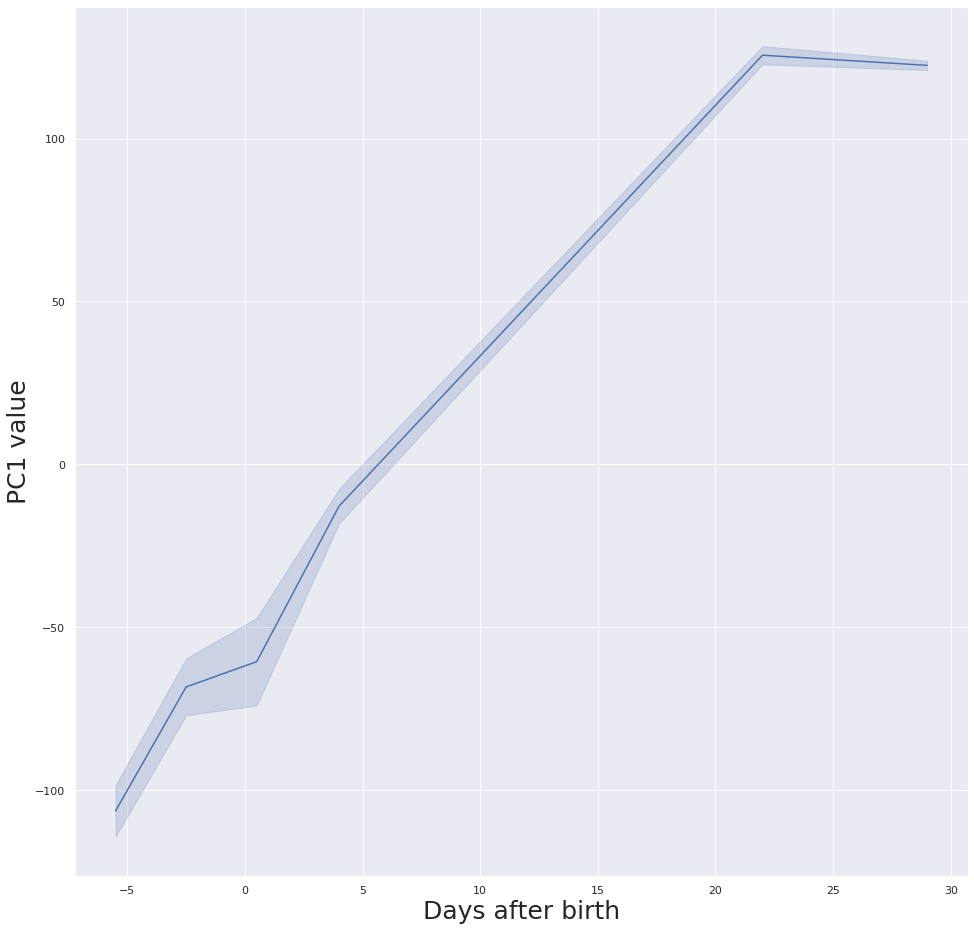
\includegraphics[width=5.5cm,height=5.5cm]{Figures&amp;Cover/Fulldata_brain_NonePCremoved_filtering_False.png}
    \caption{\textbf{The first \ac{PC} of the full sets of unmodified data from liver (left) and brain (right) as functions of age of the mice.} A very similar pattern was observed in both organs.}
    \label{fig:firstPC}
\end{figure}
\vspace{2cm}
\noindent The question then became if there was way to look past this general trend and remove the bias in the data on a global level, so variations related to specific \acp{TF} could be identified. For this purpose, \ac{PCA} was once again utilized in an attempt to remove a possible linear confounder. The data was decomposed into its \acp{PC} and then reconstructing with all but the first \ac{PC}, that encapsulated the general trend and hopefully the full effect of the confounder. When redoing the previous tests with this modified data, the similarities between the estimated activity of different \acp{TF} was overall reduced, as again exemplified with Sox11 in Figure \ref{fig:est_1PCsRemoved_Sox11}. The new estimations for all 17 \acp{TF}' activities in brain can be seen in Figure \ref{fig:BrainEstsClean1} and \ref{fig:BrainEstsClean2} in the appendix, and the estimations for their activities in liver can be seen in Figure \ref{fig:LiverEstsClean1} and \ref{fig:LiverEstsClean2} in the appendix. This was not a major concern as the correlation was expected to be far from perfect. Improvements was also seen in other cases, such as with the estimation for Satb2 as seen in Figure \ref{fig:est_1PCRemoved_Satb2}, that after the modification of the data had a similar shape to that of its gene's mRNA expression. The primary concern was however that, though less obvious, the estimations for the different \acp{TF} still appeared to follow a general trend that was also present in the mRNA expression curves. 

\begin{figure}
    \centering
    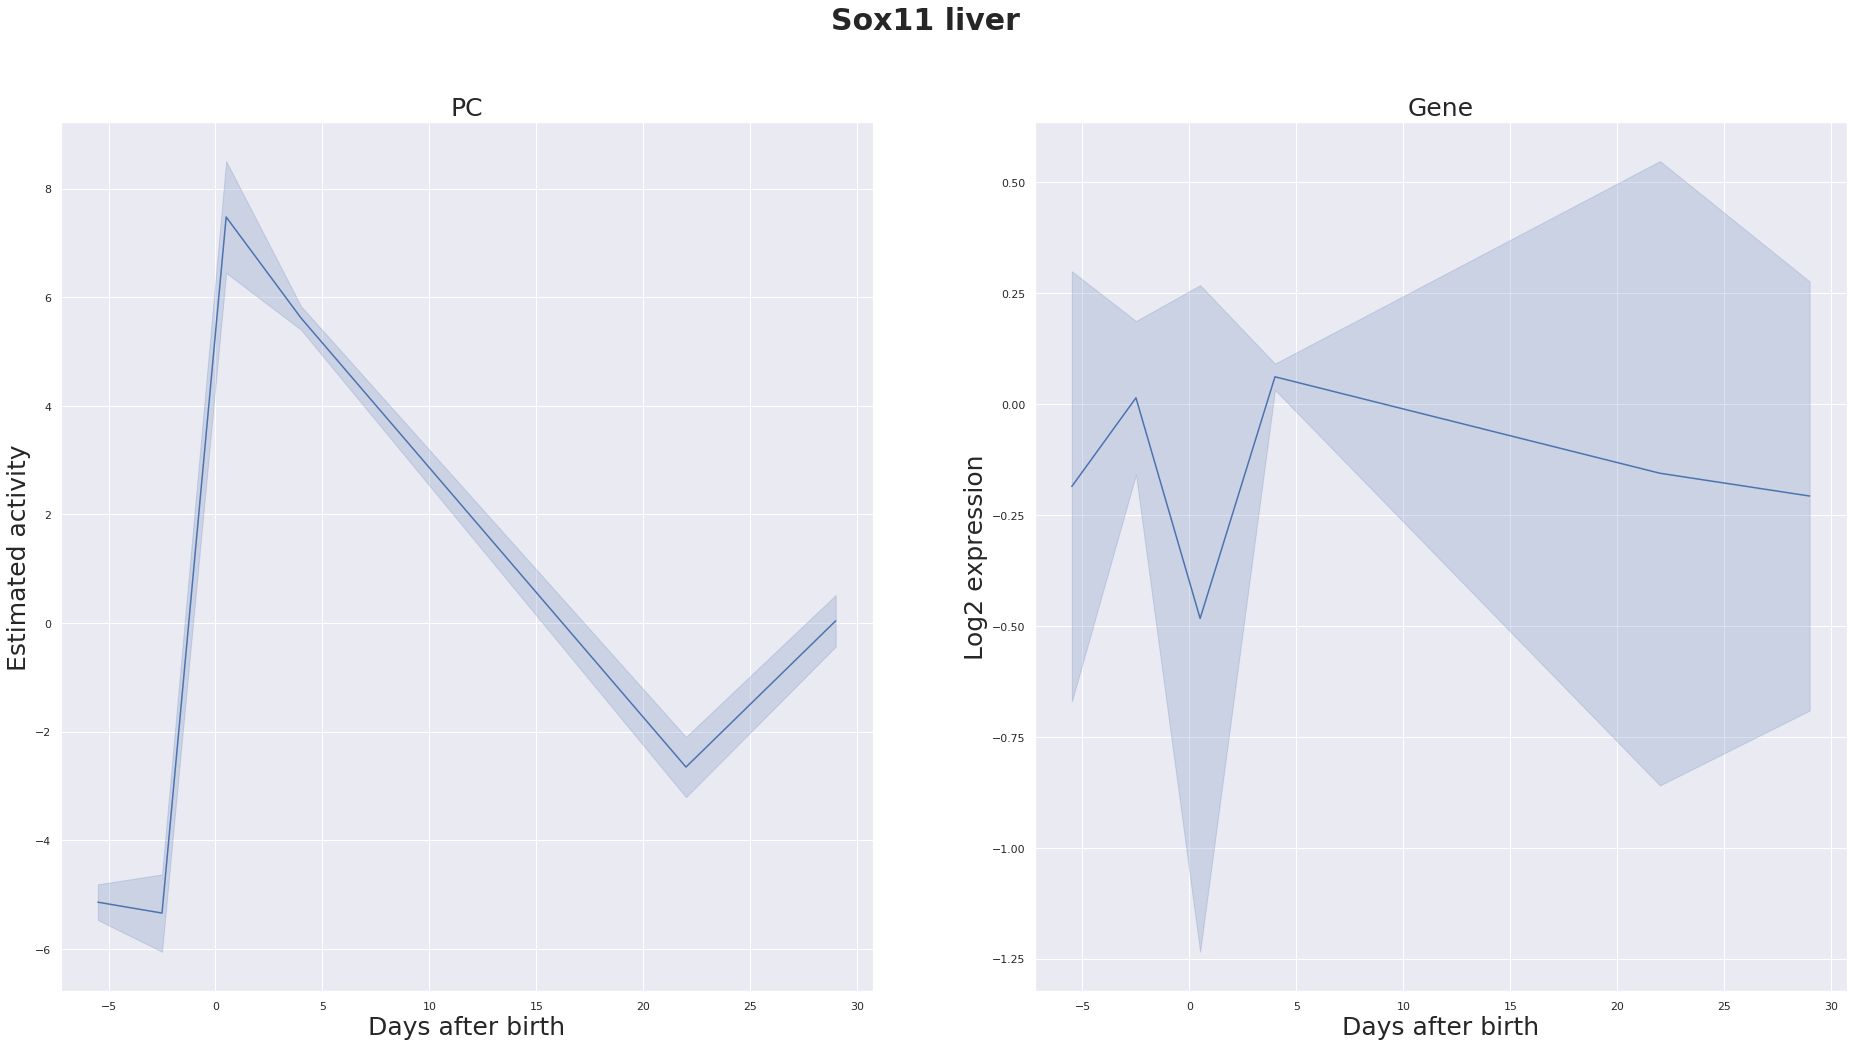
\includegraphics[width=11cm, height=5.5cm]{Figures&amp;Cover/Activity_Sox11_liver_1PCremoved_filtering_False.png}
    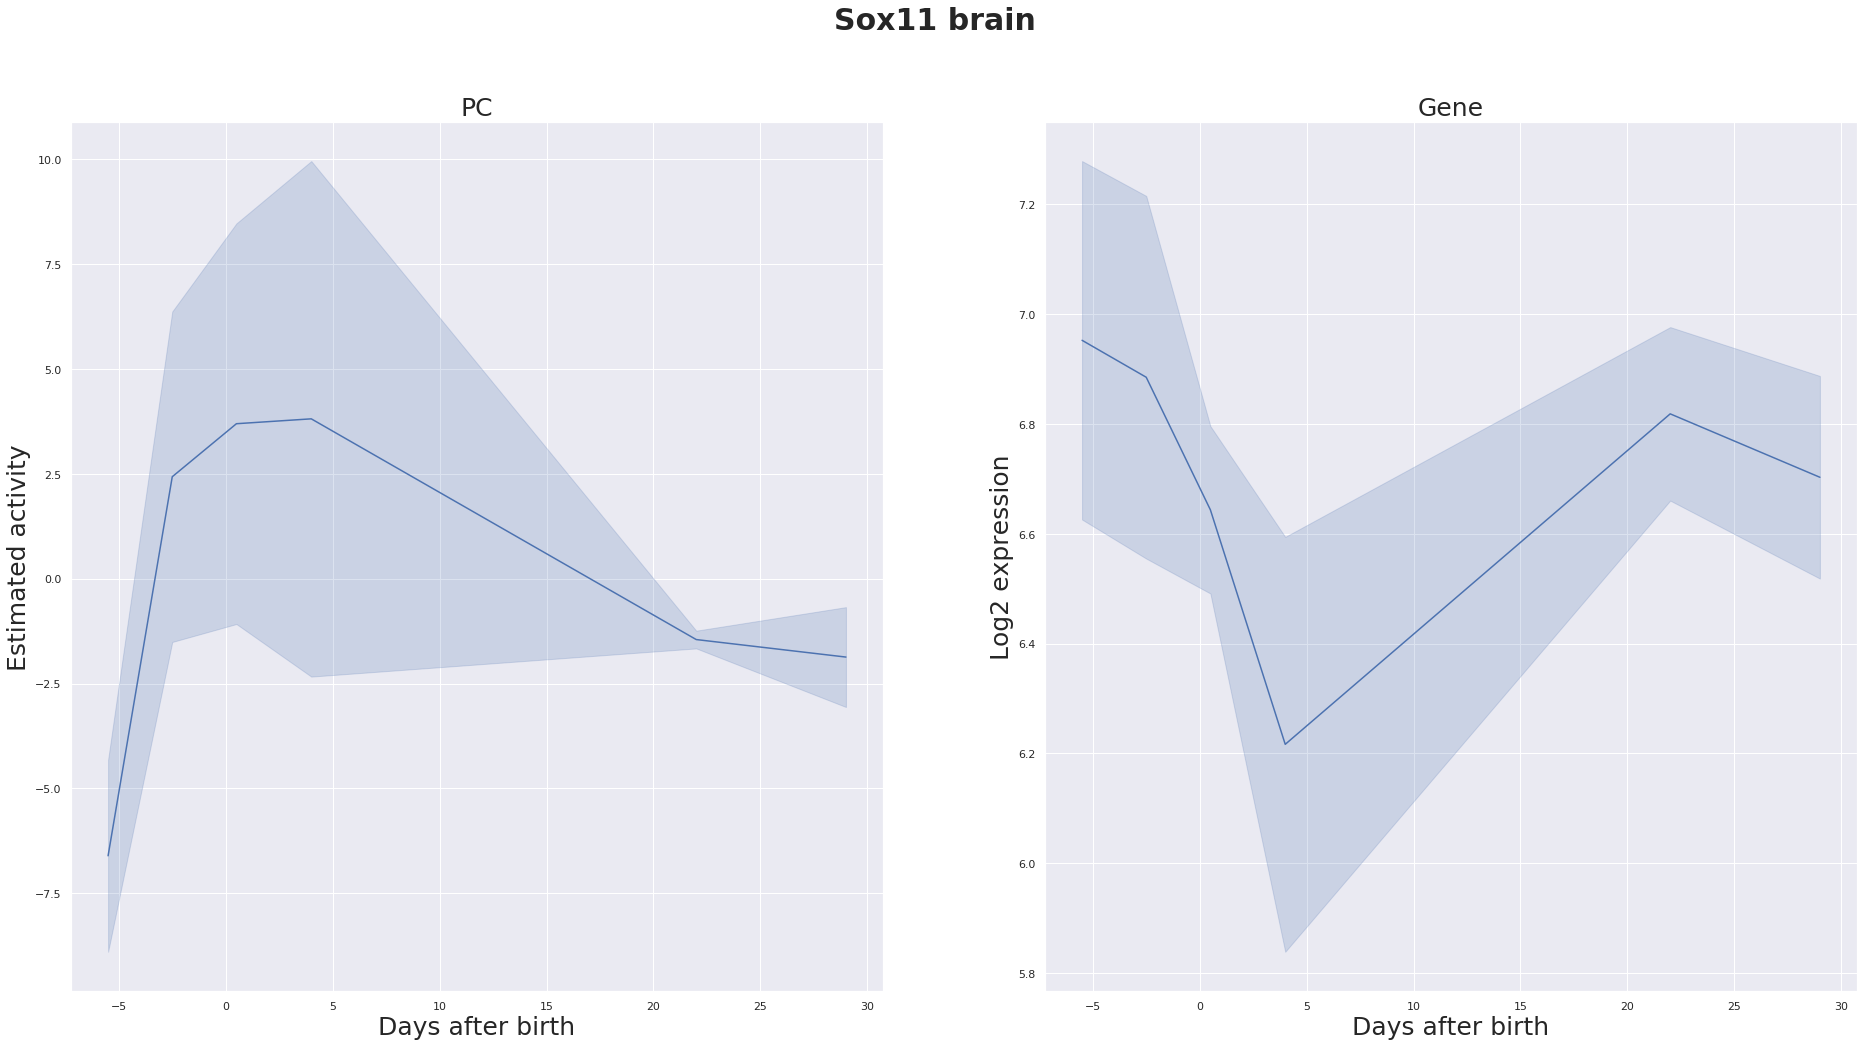
\includegraphics[width=11cm, height=5.5cm]{Figures&amp;Cover/Activity_Sox11_brain_1PCremoved_filtering_False.png}
    \caption{\textbf{Sox11's estimated activity as a functions of mices' age.} Sox11's activity was estimated by the first \ac{PC} of the mRNA expression data of the genes it is likely to regulate (upper and lower left) as well as directly through the transcription of the genes coding for it, as log2-transformed gene count (upper and lower right). The activity estimations and mRNA expressions are from the data from mouse liver (upper left and right) and brain (lower left and right) where the first \ac{PC} of the data had been removed.}
    \label{fig:est_1PCsRemoved_Sox11}
\end{figure}

\begin{figure}
    \centering
    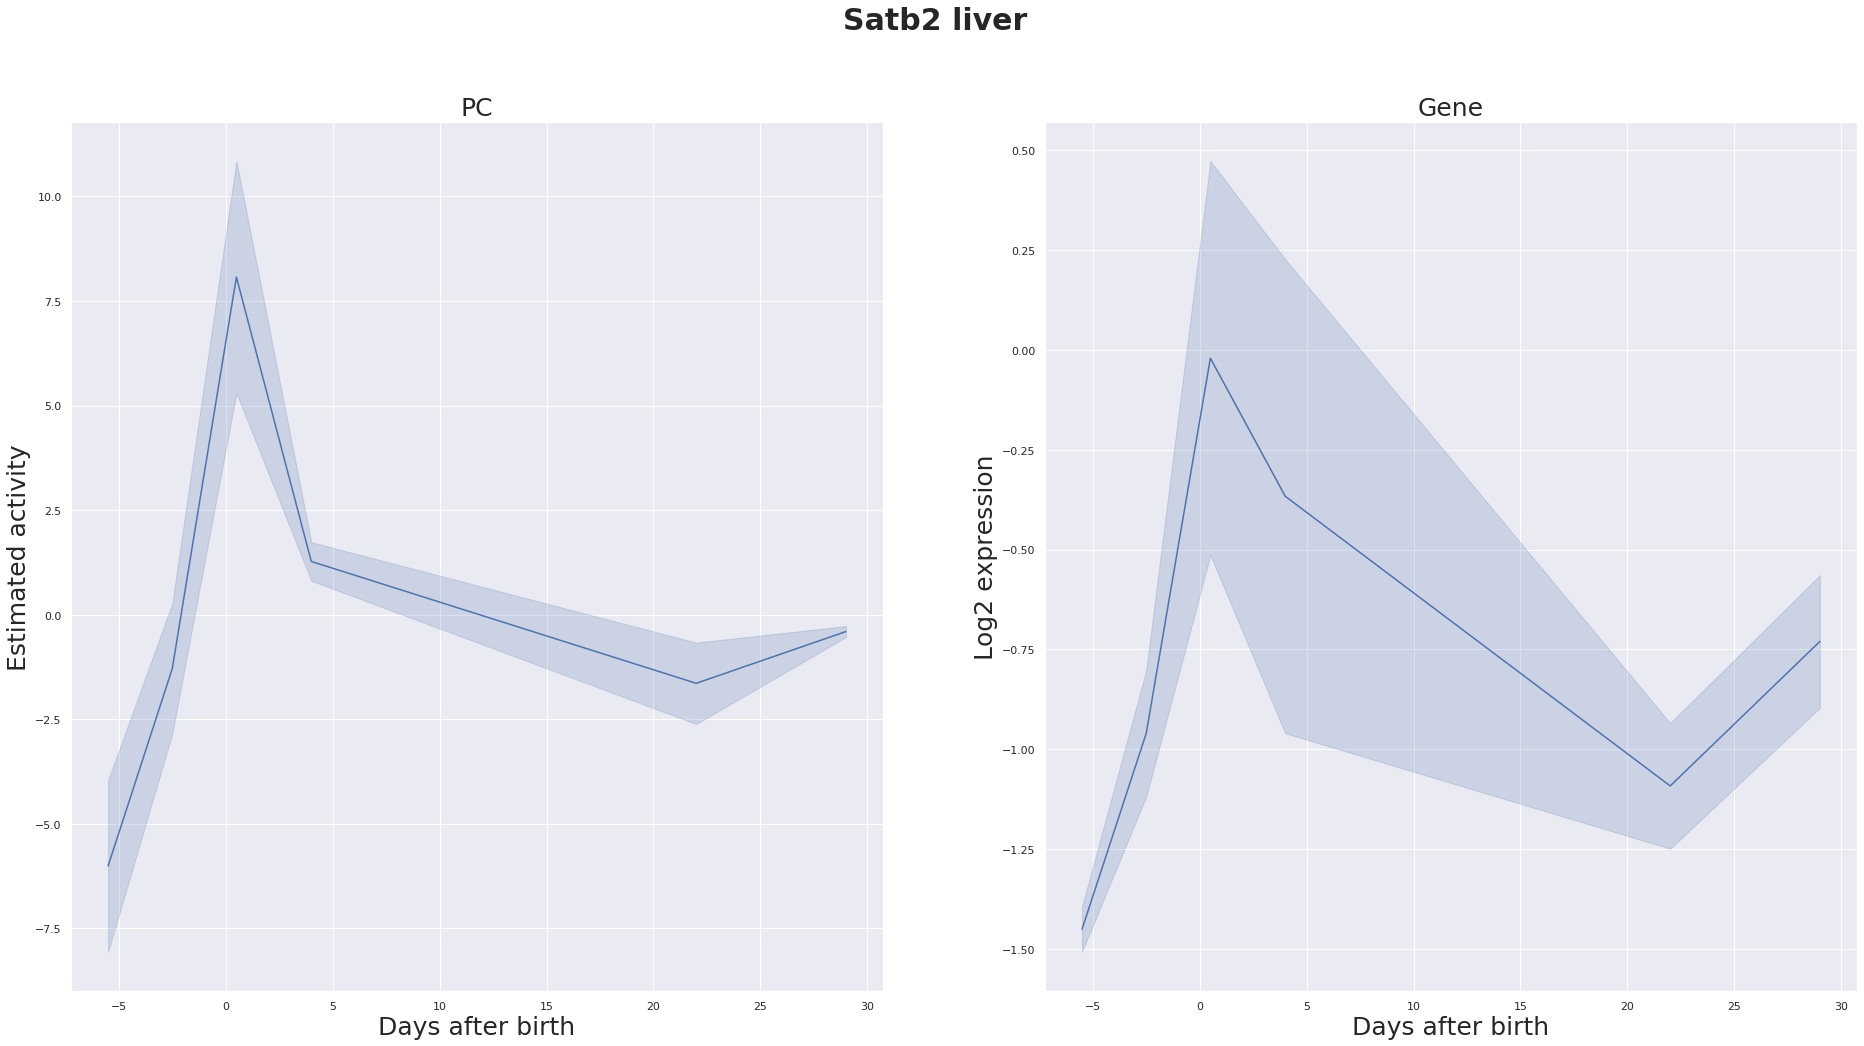
\includegraphics[width=11cm, height=5.5cm]{Figures&amp;Cover/Activity_Satb2_liver_1PCremoved_filtering_False.png}
    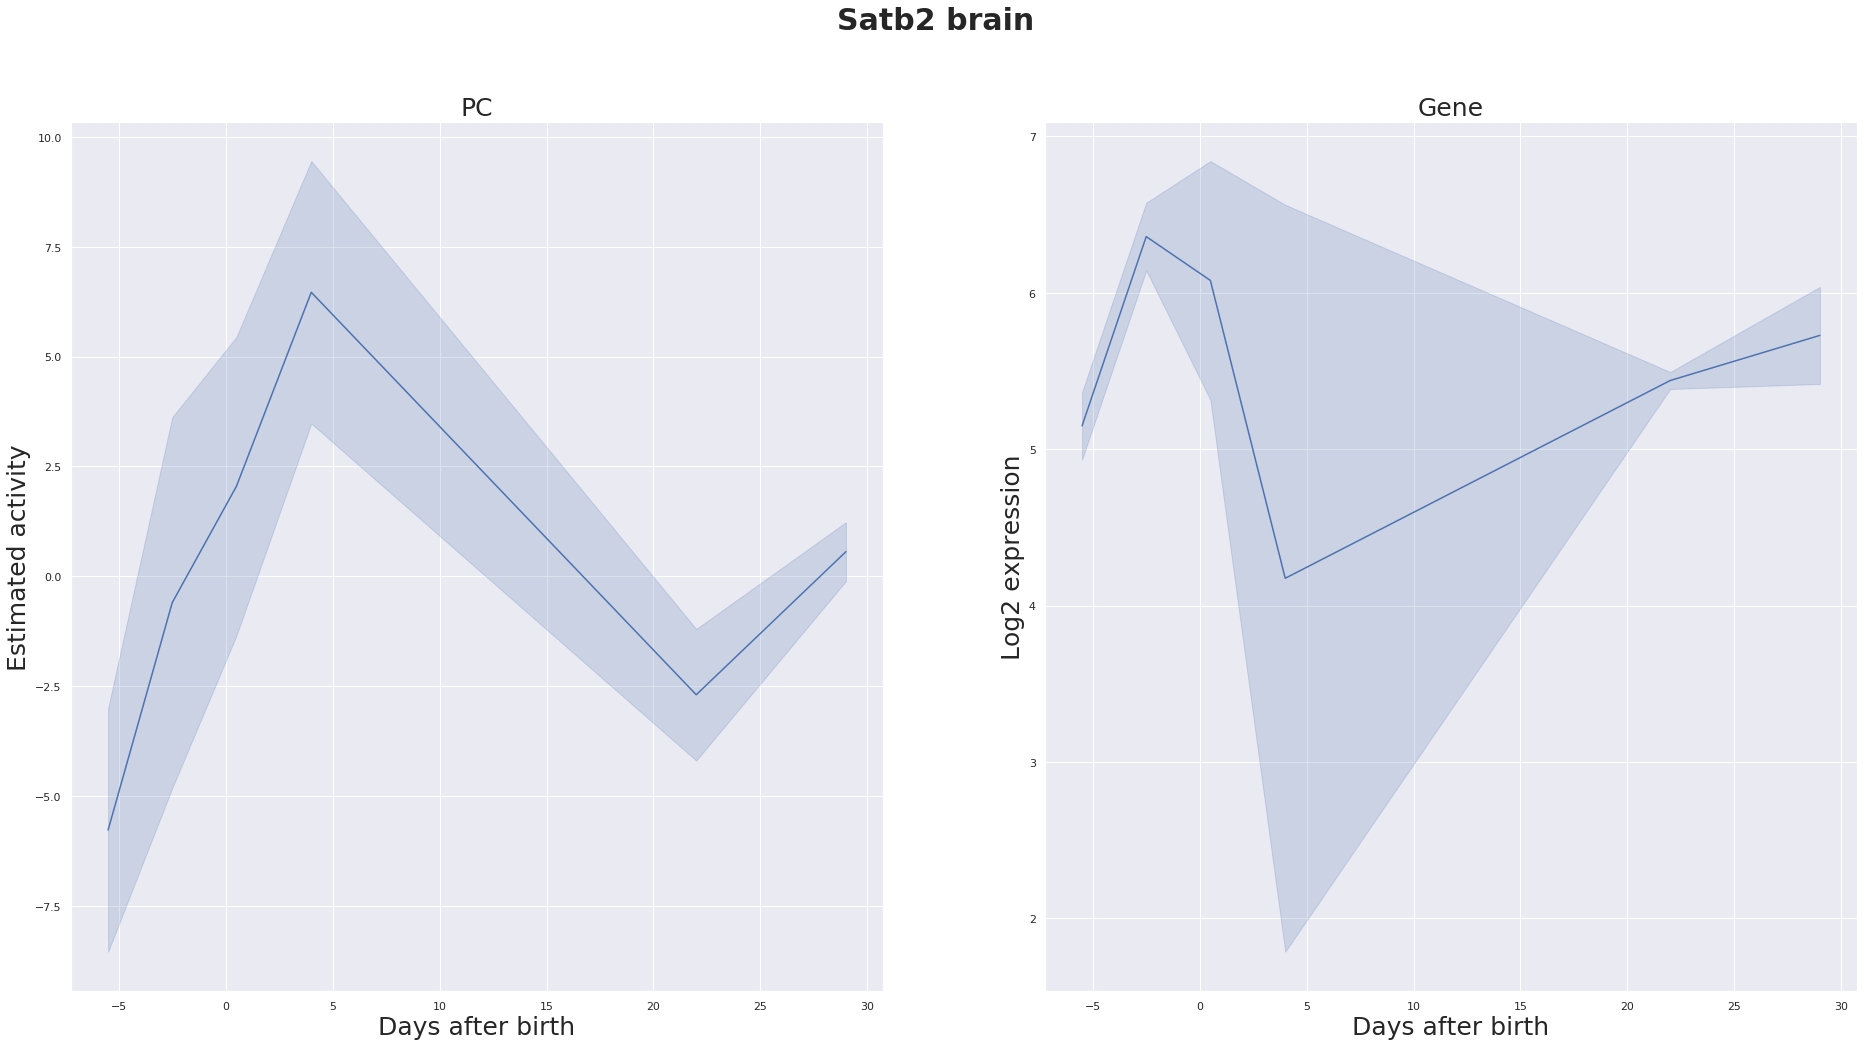
\includegraphics[width=11cm, height=5.5cm]{Figures&amp;Cover/Activity_Satb2_brain_1PCremoved_filtering_False.png}
    \caption{\textbf{Satb2's estimated activity as a functions of mices' age.} Satb2's activity was estimated by the first \ac{PC} of the mRNA expression data of the genes it is likely to regulate (upper and lower left) as well as directly through the transcription of the genes coding for it, as log2-transformed gene count (upper and lower right). The activity estimations and mRNA expressions are from the data from mouse liver (upper left and right) and brain (lower left and right) where the first \ac{PC} of the data had been removed.}
    \label{fig:est_1PCRemoved_Satb2}
\end{figure}

When the percentage of total variance explained by the \ac{PC} used as activity estimation for each \ac{TF} was plotted for the modified data it was reveled that it clustered around 35\%, but with slightly higher values for smaller gene sets, as can be seen in Figure \ref{fig:VarExp_1PCsRemoved}. This was an overall decrease of about 25 percentage points and showed that the attempt to remove the general trend had had an effect on reducing the similarities between the patterns of mRNA expression of different genes. Comparing the variance explained before and after the modification of the data gave an approximate size estimate of the linear part of the confounding effects that were removed. The results from plotting the first \ac{PC} of the complete modified data set, which is equivalent to the second \ac{PC} of the unmodified data set, can be seen in Figure \ref{fig:firstPCremoved}. The curves for the different organs were again highly similar, and when compared to the activity estimations a common, though this time much less clear, pattern could still be observed.

\begin{figure}
    \centering
    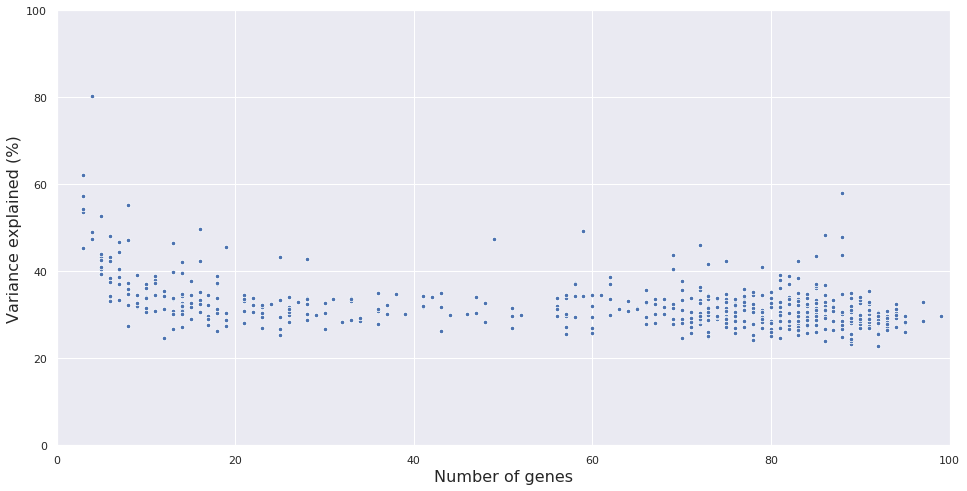
\includegraphics[width=10cm,height=5cm]{Figures&amp;Cover/VarExpl_PC1_10_300_100_liver_1PCremoved_filtering_False.png}
    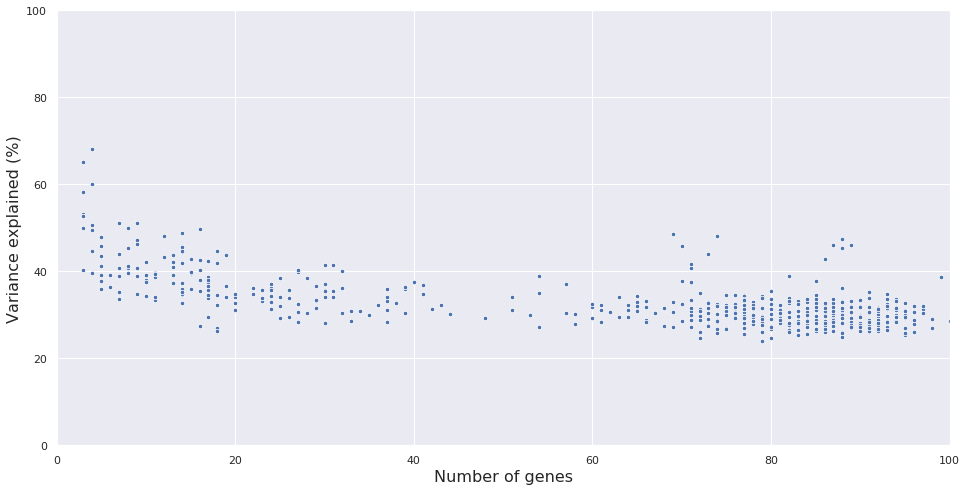
\includegraphics[width=10cm,height=5cm]{Figures&amp;Cover/VarExpl_PC1_10_300_100_brain_1PCremoved_filtering_False.png}
    \caption{\textbf{The variance explained in the transcription data of the genes in each \ac{TF}'s gene set, as a function of the number of genes in the gene set, after the data had been modified.} For the top plot the modified data from mouse liver was used and for the bottom plot the modified data from mouse brain. For both data sets, the first \ac{PC} explained about 35\% of the variance, slightly more for smaller gene sets. Comparing this to the variance explained in the gene sets with unmodified data (Figure \ref{fig:VarExp_allPCs}), where about 60\% of the variance was explained, gives an approximate size estimate of the linear part of the confounding effects that were removed.}
    \label{fig:VarExp_1PCsRemoved}
\end{figure}

\begin{figure}
    \centering
    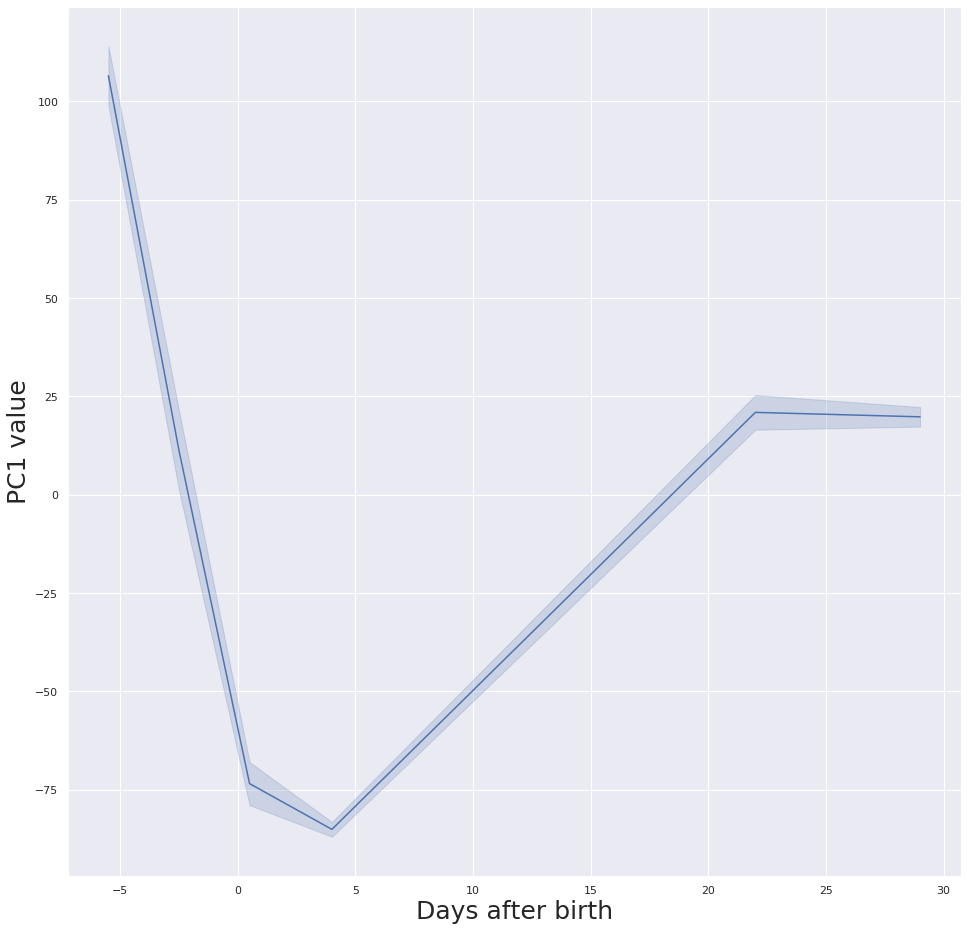
\includegraphics[width=5.5cm,height=5.5cm]{Figures&amp;Cover/Fulldata_liver_1PCremoved_filtering_False.png}
    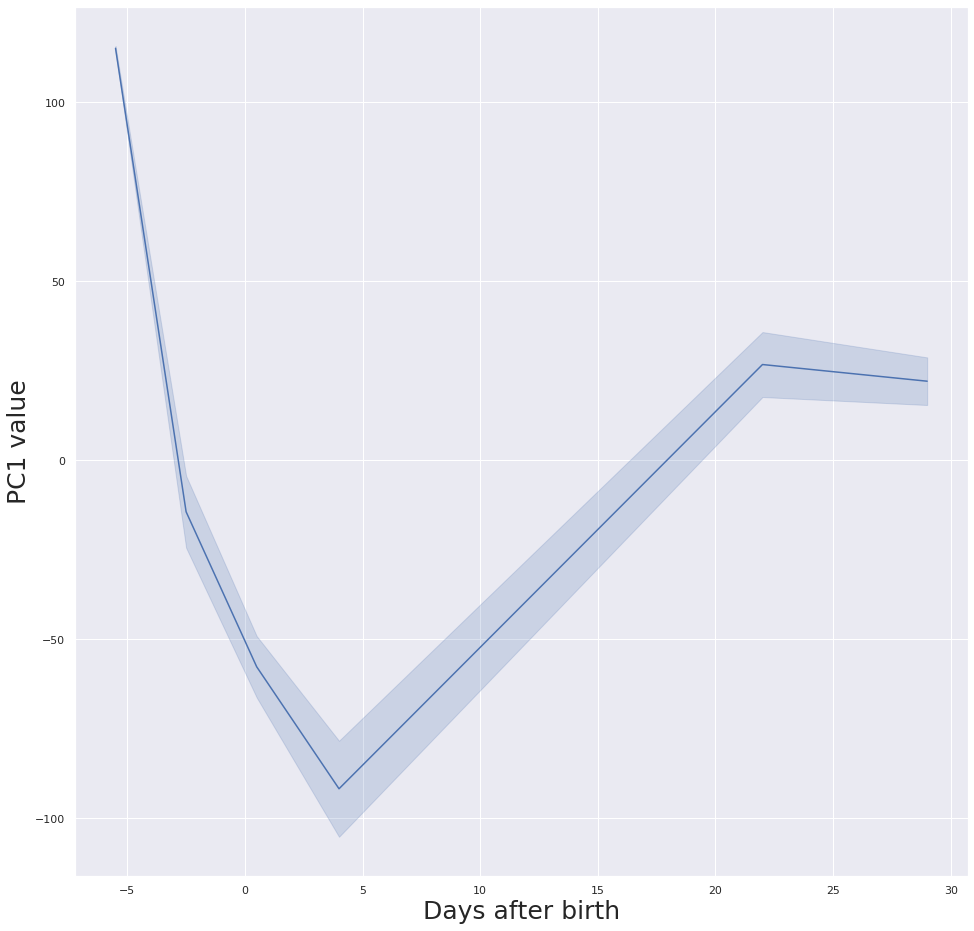
\includegraphics[width=5.5cm,height=5.5cm]{Figures&amp;Cover/Fulldata_brain_1PCremoved_filtering_False.png}
    \caption{\textbf{The first \acp{PC} of the full sets of modified data from liver (left) and brain (right) as functions of age of the mice.} The data was modified by removing the first \ac{PC} prior to analysis, meaning that this is equivalent to the second principal component for the unmodified data.}
    \label{fig:firstPCremoved}
\end{figure}



